\chapter{Odpowiedzi skokowe i charakterystyka statyczna}

\section{Wyznaczenie dpowiedzi skokowych}
W celu wyznaczenia odpowiedzi skokowych obiekt pobudzony zosta� czterema skokami sygna�u steruj�cego w chwili k=21. Sygna� steruj�cy zmienia� si� o $dU$=0,1 od $U_{min}$=0,9 do $U_{max}$=1,3.

\begin{figure}[h!]
\centering
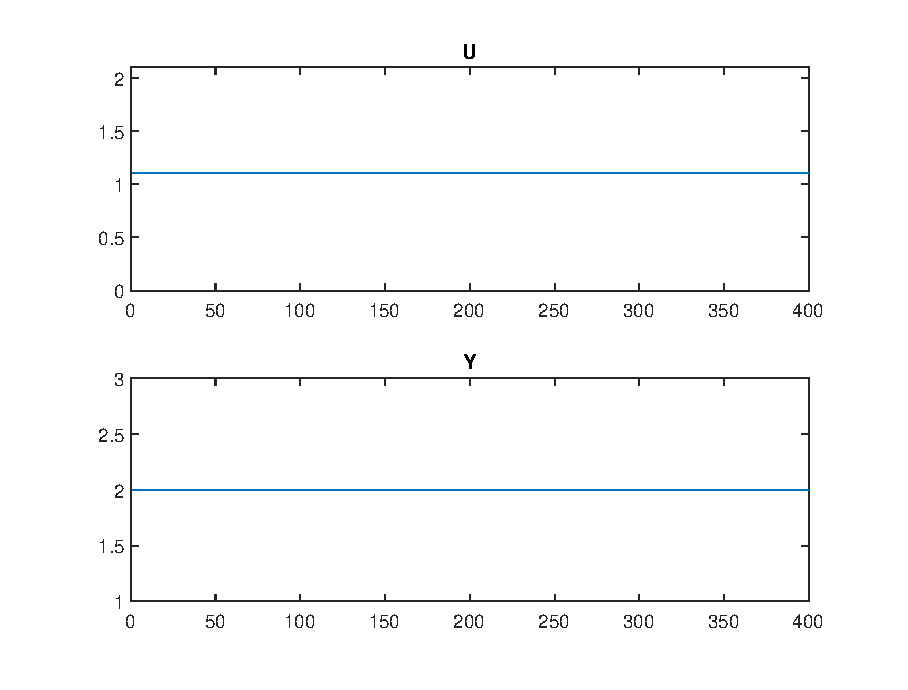
\includegraphics[scale=0.5]{rysunki/p1.eps}
\caption{Odpowiedzi skokowe}
\end{figure}

\section{Charakterystyka statyczna}
W celu wyznaczenia charakterystyki statycznej procesu zebrano odpowied� uk�adu dla pobudze� r�nymi warto�ciami sygna�u steruj�cego.

\begin{figure}[h!]
\centering
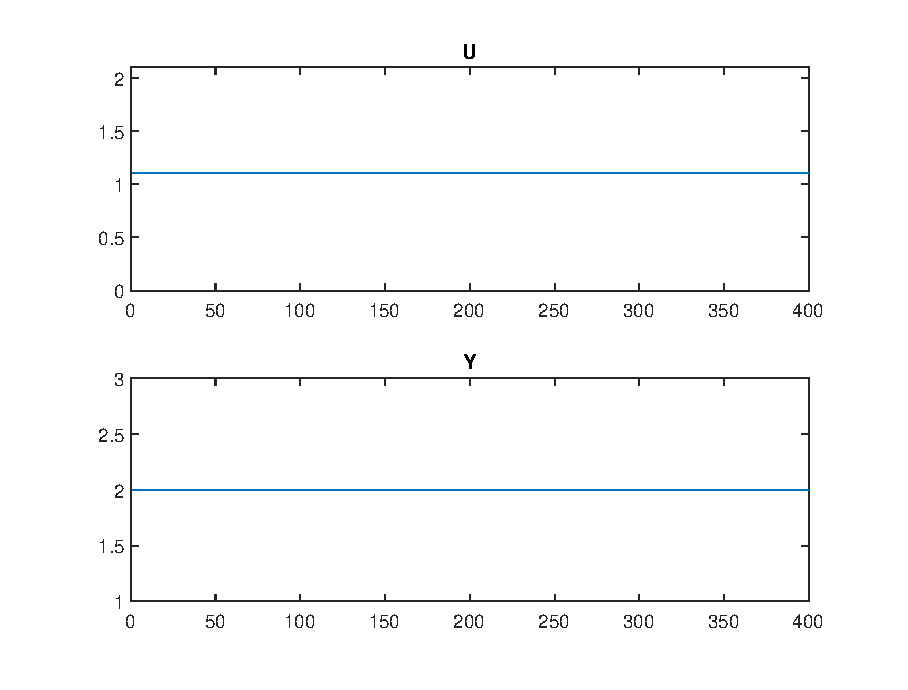
\includegraphics[scale=0.5]{rysunki/p1.eps}
\caption{Charakterystyka statyczna}
\end{figure}

\section{Wnioski}
Na podstawie charakterystyki statycznej mo�na powiedzie�, �e obiekt jest w przybli�eniu liniowy. Mo�na zatem wyznaczy� wzmocnienie statyczne procesu na podstawie wzoru:

\begin{equation}
K_{stat} = \frac{\Delta y}{\Delta u}
\end{equation}

Dla danego procesu wzmocnienie statyczne wynosi $K$ = 3,178.

\section{Implementacja}
Implementacja fukcji wykorzystanych do wykonania zadania zawarte s� w skrypcie \verb+podpunkt_2_v1.m+.